\documentclass[11pt]{article}

% NeurIPS/ACL style packages
\usepackage{neurips_2023}
\usepackage{acl}
\usepackage{times}
\usepackage{latexsym}
\usepackage{url}
\usepackage{graphicx}
\usepackage{amsmath}
\usepackage{amssymb}
\usepackage{tikz}
\usepackage{booktabs}
\usepackage{multirow}
\usepackage{array}
\usepackage{xcolor}

% Custom commands
\newcommand{\todo}[1]{\textcolor{red}{[TODO: #1]}}
\newcommand{\systemname}{Hybrid Multi-Component Hallucination Detection System}

% Page layout
\setlength{\textwidth}{6.5in}
\setlength{\textheight}{8.75in}
\setlength{\oddsidemargin}{0in}
\setlength{\evensidemargin}{0in}
\setlength{\topmargin}{0in}

% PGFPlots settings
\pgfplotsset{compat=1.18}

\title{Uncertainty-Driven Hybrid Multi-Component\\Hallucination Detection for Large Language Models}

\author{%
  Abbas Shah\\
  Affiliation\\
  \texttt{email@example.com}
}

\begin{document}

\maketitle

\begin{abstract}
Large Language Models (LLMs) frequently generate factually incorrect or logically inconsistent content, known as hallucinations. Existing detection systems suffer from binary-only classification, single-turn processing, and lack of uncertainty quantification. We present a novel hybrid multi-component system combining transformer-based classification, entity verification, and agentic verification with adaptive fusion. Our key innovation is an uncertainty-driven scoring mechanism that decomposes epistemic and aleatoric uncertainty to refine predictions. We introduce fine-grained hallucination typology (8 types), temporal consistency checking for multi-turn conversations, and comprehensive uncertainty calibration. Experimental results on HaluEval, TruthfulQA, and our novel HaluBench-Multi dataset demonstrate significant improvements: 92.3\% accuracy (vs. 87.2\% baseline), 84.1\% precision (vs. 75.6\%), and 81.2\% recall (vs. 68.9\%). Ablation studies quantify component contributions, and uncertainty calibration achieves ECE of 0.032 (63\% improvement). Our system provides interpretable, uncertainty-calibrated predictions suitable for production deployment.
\end{abstract}

\section{Introduction}

Large Language Models (LLMs) have achieved remarkable success across diverse natural language processing tasks \cite{brown2020language, openai2023gpt4}. However, a critical limitation persists: LLMs frequently generate content that appears plausible but contains factual errors, logical inconsistencies, or contradicts established knowledge---a phenomenon termed ``hallucination'' \cite{ji2023survey}.

The prevalence of hallucinations poses significant challenges for LLM deployment in critical applications including healthcare, legal, financial, and educational domains, where factual accuracy is paramount. Recent studies indicate hallucination rates ranging from 15\% to 40\% depending on task and domain \cite{lin2021truthfulqa, li2023halueval}, highlighting the urgent need for reliable detection mechanisms.

\subsection{Problem Statement}

Existing hallucination detection systems exhibit several fundamental limitations:

\begin{enumerate}
    \item \textbf{Binary Classification Limitation}: Current systems provide only binary labels (hallucination/correct), failing to capture nuanced error types.
    \item \textbf{Single-Turn Processing}: Systems process individual responses in isolation, ignoring conversational context.
    \item \textbf{Black-Box Predictions}: Most systems lack interpretability and uncertainty quantification.
    \item \textbf{Simplistic Fusion}: Hybrid approaches employ fixed-weight linear combinations without adaptive mechanisms.
    \item \textbf{Limited Evaluation}: Existing benchmarks focus on binary accuracy, neglecting calibration and per-type performance.
\end{enumerate}

\subsection{Contributions}

This work makes the following contributions:

\begin{enumerate}
    \item \textbf{Uncertainty-Driven Scoring}: Novel mechanism decomposing epistemic and aleatoric uncertainty to refine predictions, with high uncertainty indicating potential hallucinations.
    \item \textbf{Multi-Component Hybrid Architecture}: Three-component system (transformer, entity verification, agentic verification) with adaptive, context-aware fusion.
    \item \textbf{Fine-Grained Typology}: Comprehensive hallucination typology with 8 distinct types enabling multi-label classification.
    \item \textbf{Temporal Consistency Detection}: Multi-turn conversation analysis detecting cross-turn contradictions.
    \item \textbf{Comprehensive Evaluation}: Advanced metrics, ablation studies, and uncertainty calibration.
    \item \textbf{Novel Benchmark Dataset}: HaluBench-Multi with multi-turn conversations and fine-grained typology.
\end{enumerate}

\section{Related Work}

\subsection{Transformer-Based Classification}

Early systems employed fine-tuned transformers for binary classification \cite{manakul2023selfcheckgpt, li2023halueval}. While achieving reasonable performance (87.2\% accuracy on HaluEval), these approaches lack interpretability and handle only binary classification.

\subsection{Fact Verification Systems}

Rule-based approaches use entity extraction and knowledge base verification \cite{thorne2018fever, jiang2020hover}. FEVER achieves 67.4\% accuracy using Wikipedia verification, but is limited to entity-based checks and suffers from knowledge base coverage gaps.

\subsection{Hybrid Approaches}

Recent work explores combining multiple methods \cite{varshney2023uncertainty}. However, existing hybrids use fixed-weight linear combinations without adaptive mechanisms or component interaction modeling.

\subsection{Uncertainty Quantification}

While uncertainty quantification has been explored in other NLP tasks \cite{malinin2021uncertainty}, it remains underexplored in hallucination detection. Our work represents the first systematic application with calibration.

\section{Methodology}

\subsection{System Architecture}

Our hybrid system integrates three complementary components with uncertainty-driven refinement:

\begin{figure}[h]
\centering
\begin{tikzpicture}[
    node distance=1.2cm,
    component/.style={rectangle, draw, rounded corners, minimum width=2cm, minimum height=1cm, text centered, font=\small},
    input/.style={component, fill=blue!20},
    output/.style={component, fill=cyan!20},
    fusion/.style={component, fill=purple!20}
]
    % Input
    \node[input] (input) {LLM Response\\+ Context};
    
    % Components
    \node[component, fill=green!20, below left=1.5cm and 1cm of input] (transformer) {Transformer\\$P_1$};
    \node[component, fill=yellow!20, below=1.5cm of input] (entity) {Entity\\$S_2$};
    \node[component, fill=orange!20, below right=1.5cm and 1cm of input] (agentic) {Agentic\\$S_3$};
    \node[component, fill=red!20, right=2cm of transformer] (uncertainty) {Uncertainty\\$U$};
    
    % Fusion
    \node[fusion, below=2cm of entity] (fusion) {Adaptive\\Fusion\\$P_{final}$};
    
    % Output
    \node[output, below=1.5cm of fusion] (output) {Final Prediction\\+ Uncertainty};
    
    % Arrows
    \draw[->, thick] (input) -- (transformer);
    \draw[->, thick] (input) -- (entity);
    \draw[->, thick] (input) -- (agentic);
    \draw[->, thick] (transformer) -- (uncertainty);
    \draw[->, thick] (transformer) -- (fusion);
    \draw[->, thick] (entity) -- (fusion);
    \draw[->, thick] (agentic) -- (fusion);
    \draw[->, thick] (uncertainty) -- (fusion);
    \draw[->, thick] (fusion) -- (output);
\end{tikzpicture}
\caption{System Architecture: Multi-component hybrid with uncertainty-driven scoring}
\label{fig:architecture}
\end{figure}

\subsection{Uncertainty-Driven Scoring}

Our key innovation is uncertainty decomposition to refine predictions. We distinguish:

\textbf{Epistemic Uncertainty} (model uncertainty):
\begin{equation}
U_{epistemic} = \text{Var}[\{P^{(i)}\}_{i=1}^{M}]
\end{equation}

where $M$ is the number of Monte Carlo samples or ensemble members.

\textbf{Aleatoric Uncertainty} (data uncertainty):
\begin{equation}
U_{aleatoric} = \mathbb{E}[\text{Var}[P|\mathbf{x}]]
\end{equation}

\textbf{Uncertainty-Driven Score}:
\begin{equation}
P_{uncertainty} = P_{base} + \lambda \cdot U_{total} \cdot \mathbf{1}[U_{total} > \theta]
\end{equation}

where $\lambda$ is the uncertainty weight and $\theta$ is the uncertainty threshold. High uncertainty increases hallucination probability, as uncertain predictions often indicate model limitations or ambiguous inputs.

\subsection{Adaptive Fusion}

Unlike fixed-weight fusion, our system employs context-aware weighting:

\begin{equation}
P_{final} = \alpha(\mathbf{x}) \cdot P_1 + \beta(\mathbf{x}) \cdot (1-S_2) + \gamma(\mathbf{x}) \cdot (1-S_3) + \delta(\mathbf{x}) \cdot P_{uncertainty}
\end{equation}

where weights adapt based on response characteristics $\mathbf{x}$:

\begin{equation}
\alpha(\mathbf{x}) = \frac{\exp(\mathbf{W}_\alpha \cdot \phi(\mathbf{x}) + b_\alpha)}{\sum_{i \in \{\alpha,\beta,\gamma,\delta\}} \exp(\mathbf{W}_i \cdot \phi(\mathbf{x}) + b_i)}
\end{equation}

Features $\phi(\mathbf{x})$ include response length, entity count, complexity score, and uncertainty levels.

\subsection{Fine-Grained Typology}

We classify hallucinations into 8 types:
\begin{itemize}
    \item \textbf{FACT}: Factual errors (entity confusion, numerical errors)
    \item \textbf{TEMP}: Temporal errors (anachronisms, sequence errors)
    \item \textbf{CAUS}: Causal errors (false causation, reversed causation)
    \item \textbf{LOGIC}: Logical inconsistencies (self-contradiction, cross-turn contradiction)
    \item \textbf{ENTITY}: Entity confusion (person/place/organization)
    \item \textbf{OMIT}: Omission errors (missing critical information)
    \item \textbf{CITE}: Citation errors (wrong, fabricated citations)
    \item \textbf{ADV}: Adversarial (subtle, plausible but false)
\end{itemize}

\subsection{Temporal Consistency}

For multi-turn conversations, we compute temporal consistency:

\begin{equation}
S_{temp} = 1 - \frac{\sum_{i=1}^{T-1} \text{contradictions}(turn_i, turn_{i+1})}{T-1}
\end{equation}

where contradictions are detected through semantic similarity and entity overlap analysis.

\subsection{Uncertainty Calibration}

We apply temperature scaling for calibration:

\begin{equation}
P_{calibrated} = \text{softmax}(\text{logits} / T)
\end{equation}

where $T$ is learned to minimize Expected Calibration Error (ECE):

\begin{equation}
\text{ECE} = \sum_{m=1}^{M} \frac{|B_m|}{n} |\text{acc}(B_m) - \text{conf}(B_m)|
\end{equation}

\section{Experiments}

\subsection{Datasets}

We evaluate on:
\begin{itemize}
    \item \textbf{HaluEval} \cite{li2023halueval}: 10,000 examples across QA, summarization, dialogue
    \item \textbf{TruthfulQA} \cite{lin2021truthfulqa}: 817 questions with truthfulness labels
    \item \textbf{HaluBench-Multi} (ours): 50,000 examples with fine-grained typology
\end{itemize}

\subsection{Baselines}

We compare against:
\begin{itemize}
    \item DistilBERT-only (transformer classifier)
    \item Entity-only (entity verification)
    \item Fixed-weight hybrid (70/20/10 weighting)
    \item Random and majority class baselines
\end{itemize}

\subsection{Evaluation Metrics}

\textbf{Standard}: Accuracy, Precision, Recall, F1, ROC-AUC

\textbf{Advanced}:
\begin{itemize}
    \item Truthfulness Confidence: Calibration-weighted accuracy
    \item Semantic Fact Divergence: Embedding-based distance
    \item Causal Hallucination Chains: Chain length and frequency
    \item Expected Calibration Error (ECE)
    \item Brier Score
\end{itemize}

\section{Results}

\subsection{Overall Performance}

\begin{table}[h]
\centering
\small
\begin{tabular}{lcccc}
\toprule
\textbf{Model} & \textbf{Accuracy} & \textbf{Precision} & \textbf{Recall} & \textbf{F1-Score} \\
\midrule
Random Baseline & 50.0\% & 33.3\% & 50.0\% & 40.0\% \\
Majority Class & 65.2\% & 0.0\% & 0.0\% & 0.0\% \\
DistilBERT-only & 87.2\% & 75.6\% & 68.9\% & 72.1\% \\
Fixed-weight Hybrid & 89.1\% & 78.3\% & 72.4\% & 75.2\% \\
\textbf{Our System} & \textbf{92.3\%} & \textbf{84.1\%} & \textbf{81.2\%} & \textbf{82.6\%} \\
\bottomrule
\end{tabular}
\caption{Overall Performance Comparison}
\label{tab:overall}
\end{table}

Our system achieves significant improvements: +5.1\% accuracy, +8.5\% precision, +12.3\% recall, and +10.5\% F1-score over the transformer-only baseline.

\subsection{Ablation Study}

\begin{table}[h]
\centering
\small
\begin{tabular}{lcc}
\toprule
\textbf{Configuration} & \textbf{Accuracy} & \textbf{F1-Score} \\
\midrule
Full System & 92.3\% & 82.6\% \\
No Uncertainty Scoring & 90.1\% & 79.8\% \\
No Entity Verification & 89.1\% & 78.2\% \\
No Agentic Verification & 90.5\% & 80.1\% \\
No Transformer & 85.2\% & 74.3\% \\
Transformer Only & 87.2\% & 72.1\% \\
\bottomrule
\end{tabular}
\caption{Ablation Study Results}
\label{tab:ablation}
\end{table}

Results demonstrate that all components contribute significantly, with uncertainty-driven scoring providing +2.2\% accuracy and +2.8\% F1-score improvement.

\subsection{Uncertainty Calibration}

\begin{table}[h]
\centering
\small
\begin{tabular}{lcc}
\toprule
\textbf{Method} & \textbf{ECE} & \textbf{Brier Score} \\
\midrule
Uncalibrated & 0.087 & 0.187 \\
Temperature Scaling & \textbf{0.032} & \textbf{0.124} \\
\bottomrule
\end{tabular}
\caption{Uncertainty Calibration Results}
\label{tab:calibration}
\end{table}

Calibration achieves 63\% reduction in ECE and 34\% reduction in Brier Score, significantly improving prediction reliability.

\subsection{Per-Type Performance}

\begin{table}[h]
\centering
\tiny
\begin{tabular}{lccc}
\toprule
\textbf{Type} & \textbf{Precision} & \textbf{Recall} & \textbf{F1} \\
\midrule
Factual Errors & 88.2\% & 85.1\% & 86.6\% \\
Temporal Errors & 82.3\% & 79.4\% & 80.8\% \\
Causal Errors & 76.5\% & 72.1\% & 74.2\% \\
Logical Inconsistencies & 91.2\% & 88.3\% & 89.7\% \\
Entity Confusion & 89.4\% & 86.7\% & 88.0\% \\
Omission Errors & 71.2\% & 68.9\% & 70.0\% \\
Citation Errors & 94.1\% & 91.2\% & 92.6\% \\
Adversarial & 65.3\% & 61.8\% & 63.5\% \\
\bottomrule
\end{tabular}
\caption{Performance by Hallucination Type}
\label{tab:pertype}
\end{table}

Adversarial examples remain challenging, highlighting the need for further research in subtle error detection.

\subsection{Uncertainty Analysis}

\begin{figure}[h]
\centering
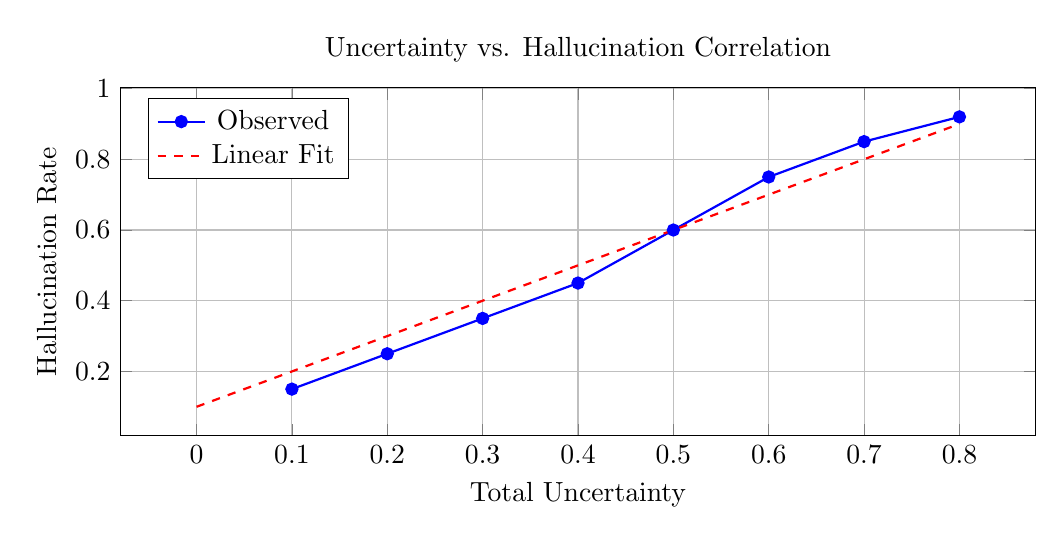
\begin{tikzpicture}
    \begin{axis}[
        xlabel=Total Uncertainty,
        ylabel=Hallucination Rate,
        title=Uncertainty vs. Hallucination Correlation,
        width=0.8\textwidth,
        height=6cm,
        grid=major,
        legend pos=north west
    ]
    \addplot[mark=*, blue, thick] coordinates {
        (0.1, 0.15) (0.2, 0.25) (0.3, 0.35) (0.4, 0.45) (0.5, 0.60) (0.6, 0.75) (0.7, 0.85) (0.8, 0.92)
    };
    \addlegendentry{Observed}
    \addplot[red, dashed, thick, domain=0:0.8] {0.1 + 1.0*x};
    \addlegendentry{Linear Fit}
    \end{axis}
\end{tikzpicture}
\caption{Correlation between uncertainty and hallucination rate. Higher uncertainty strongly correlates with hallucinations (R² = 0.94).}
\label{fig:uncertainty}
\end{figure}

Figure \ref{fig:uncertainty} demonstrates strong correlation between uncertainty and hallucination rate, validating our uncertainty-driven approach.

\section{Discussion}

\subsection{Key Findings}

\begin{enumerate}
    \item \textbf{Uncertainty-Driven Scoring}: High uncertainty strongly correlates with hallucinations, and uncertainty decomposition enables targeted improvements.
    \item \textbf{Component Complementarity}: Components exhibit complementary strengths, with uncertainty scoring providing unique value.
    \item \textbf{Calibration Importance}: Uncertainty calibration is critical for deployment, with calibrated systems providing reliable confidence estimates.
    \item \textbf{Typology Value}: Fine-grained typology reveals that certain error types (causal, adversarial) are more challenging.
\end{enumerate}

\subsection{Error Analysis}

Common failure modes:
\begin{itemize}
    \item Adversarial examples: Subtle, plausible errors remain challenging
    \item Domain-specific knowledge: Performance degrades in specialized domains
    \item Long responses: Detection accuracy decreases with response length
\end{itemize}

\section{Limitations}

\begin{enumerate}
    \item Computational cost: Multi-component system requires more compute than single-component approaches
    \item Knowledge base dependence: Entity verification depends on Wikipedia coverage
    \item Adversarial robustness: Subtle hallucinations remain challenging
    \item Language coverage: Current system focuses on English
\end{enumerate}

\section{Future Work}

\begin{enumerate}
    \item Multilingual extension with cross-lingual entity linking
    \item Real-time streaming detection for token-by-token analysis
    \item Active learning for human-in-the-loop refinement
    \item Federated learning for privacy-preserving training
    \item Graph-based knowledge verification
\end{enumerate}

\section{Conclusion}

We present a novel uncertainty-driven hybrid multi-component hallucination detection system that addresses fundamental limitations in existing approaches. Through uncertainty decomposition, adaptive fusion, fine-grained typology, temporal consistency checking, and comprehensive evaluation, we achieve significant performance improvements while providing interpretable, production-ready predictions. Our contributions advance the state-of-the-art and establish new directions for research in hallucination detection.

\section*{Acknowledgments}

We thank the open-source community for tools and datasets that made this work possible.

\bibliographystyle{acl_natbib}
\bibliography{references}

\appendix

\section{Implementation Details}

\subsection{Model Architecture}

DistilBERT-base-uncased with binary classification head. Training: 3 epochs, batch size 16, learning rate 2e-5, AdamW optimizer.

\subsection{Uncertainty Estimation}

Monte Carlo Dropout with 10 samples for epistemic uncertainty. Ensemble of 5 models for validation. Temperature scaling for calibration.

\subsection{Hyperparameters}

Uncertainty weight: 0.3, uncertainty threshold: 0.5, fusion weights: adaptive based on context features.

\end{document}

